Monte Carlo methods (MCM) have their roots in statistical physics, where they have been used to obtain approximations to intractable integrals\cite{b24}, and have since been used in a wide array of domains. MCMs rely on repeated random sampling to obtain numerical results. The key idea is to use randomness to solve problems that might be deterministic in principle. Thus MCMs were applied to solve RL problems based on averaging sample rewards, nowadays heavily in games AI research \cite{b18,b25}. Monte Carlo tree search (MCTS) rests on two fundamental concepts of MCMs: the actual value of action may be approximated using random simulation, and these values may be used efficiently to adjust the policy towards a best-first action strategy \cite{b18}. The algorithm progressively builds a partial game tree, guided by the previous tree exploration. The tree is used to estimate the values of actions, with these estimates (particularly those most promising actions) becoming more accurate as the tree is built.

The basic algorithm works iteratively, building a search tree until a computational budget, typically time, memory, or iteration constraint, is reached. Then the search stops, and the best performing root action is returned. Each node in the search tree represents a state of the domain, and directed links to child nodes represent actions leading to subsequent states. Typical four steps (cf. Fig.~\ref{basic_MCTS}) applied per search iteration are:
\subsubsection*{Selection} Starting at root node, \textit{tree policy} is recursively applied to select optimal child nodes until a leaf node is reached. The leaf node is expandable if it represents a nonterminal state and has unexpanded and unvisited children.
\subsubsection*{Expansion} Expand the leaf node according to the available legal actions and choose one of its children. 
\subsubsection*{Simulation} Play a simulated game starting with that node according to a \textit{default policy} to produce an outcome. Sometimes this step is termed as \textit{evaluation}. 
\subsubsection*{Backpropagation} Use the results of that simulated game to update the node and its ancestors (till the root node). The simulation result is thus `backed up' (backpropagated). It does not use any policy but updates node statistics that inform future tree policy decisions. 

\begin{figure}[t]
\centerline{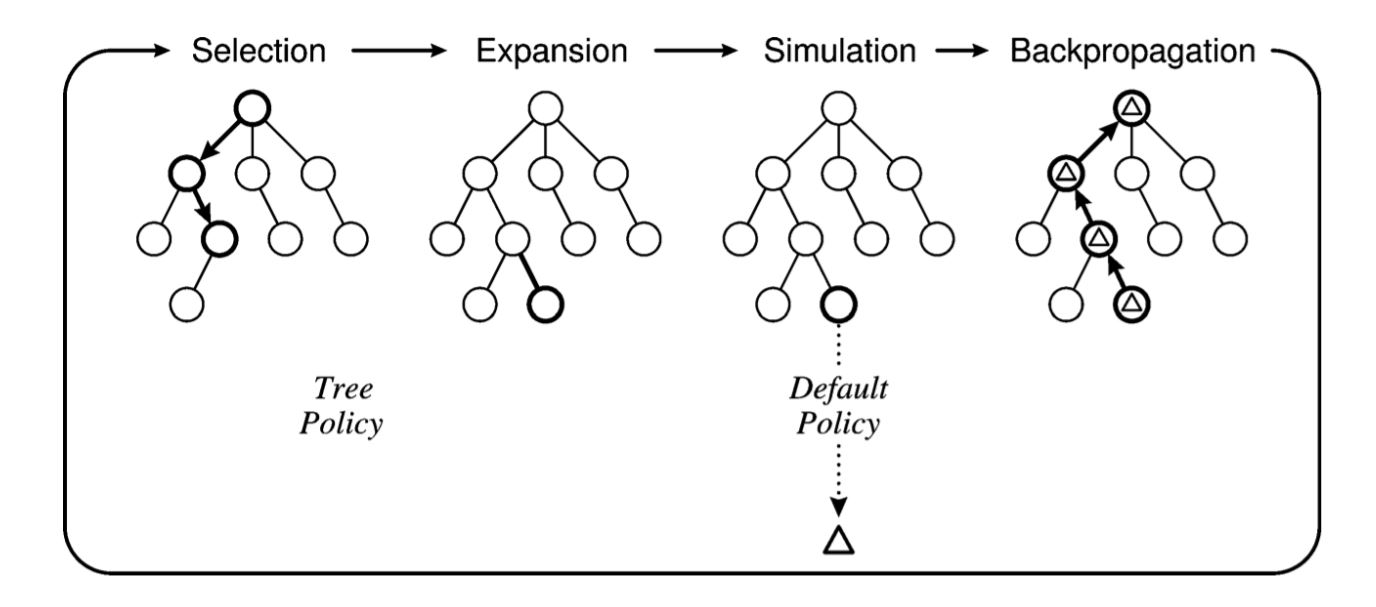
\includegraphics[width = 0.8\columnwidth]{Basic_MCTS.JPG}}
\caption{One iteration of the basic Monte Carlo tree search\cite{b18}}
\label{basic_MCTS}
\end{figure}